\section{Flavour Tagging}
\label{sec:ana_tagging}

In Chapter~\ref{chap:pheno} the expressions for the differential decay rates of $\Bs$ and $\Bsbar$ decays are distinguished by the
variable $\qf$, which takes the value \tp1 for $\Bs$ and \tm1 for $\Bsbar$. Equation~\ref{eq:timeqfDep} in Section~\ref{sec:pheno_time}
shows the dependence on this variable.

As explained in Section~\ref{subsec:intro_LHCb_LHC}, it is experimentally not possible to unambiguously determine whether the produced
meson was $\Bs$ and $\Bsbar$ for each individual decay. In practice, the meson flavour is estimated for each decay, together with a
probability that the estimate is wrong. This \emph{flavour tag} is denoted by $\qt$, which takes the values \tp1 for a $\Bs$ estimate and
\tm1 for a $\Bsbar$ estimate. The estimate of the wrong-tag probability is denoted by $\etaTag$.

For either value of $\qt$ the differential rate is a sum of the rates for true $\Bs$ ($\qf$\texteq\tp1) and true $\Bsbar$
($\qf$\texteq\tm1), where the relative contributions depend on the wrong-tag probability. For small wrong-tag probability the two
contributions are well separated, which enables the measurement of the oscillation amplitude from which the main sensitivity to
CP-violation parameters originates (see Section~\ref{subsec:pheno_equations_approx}). If the wrong-tag probability becomes larger, the
opposite oscillations of true $\Bs$ and true $\Bsbar$ start to cancel, reducing the sensitivity to the CP-violation parameters.

Decay candidates are assigned to different \emph{flavour-tagging categories} according to the estimate of the wrong-tag probability. For
the main measurement the candidates are only classified as \emph{tagged} (0\textle$\etaTag$\textlt0.5) or \emph{untagged}
($\etaTag$\texteq0.5). For tagged decay candidates the decay model depends on the value of $\etaTag$ for each candidate. For untagged
candidates the flavour-tagging algorithms are unable to estimate the $\Bs$ flavour. For these candidates the wrong-tag probability is 50\%
by definition.

Although the implementation of flavour tagging that uses the value of $\etaTag$ for each individual decay candidate is more optimal, the
analysis can be simplified by using an average wrong-tag probability for tagged candidates. In this case the tagging information can be
used more optimally by defining several categories of tagged events, such that candidates with small and large wrong-tag probabilities are
separated. This is achieved by defining ranges in $\etaTag$.

In summing the contributions of true $\Bs$ and true $\Bsbar$ any asymmetries in their production and detection should be taken into
account. The LHC collides protons, which contain more matter than antimatter. This creates a small matter--antimatter asymmetry in the
fragmentation and hadronization processes and consequently a small asymmetry in the numbers of $\Bs$ and $\Bsbar$ that are produced. In
addition, the flavour-tagging process relies on the detection of charged kaons, which is asymmetric for $\Kp$ and $\Km$. This creates a
difference in the fractions of the $\Bs$ and $\Bsbar$ decays in each tagging category.


%%%%%%%%%%%%%%%%%%%%%%%%%%%%%%%
\subsection{Formalism}
\label{subsec:ana_tagging_form}
%%%%%%%%%%%%%%%%%%%%%%%%%%%%%%%

The effect of any of $\Bs$--$\Bsbar$ normalization asymmetries on the differential decay rate can be written in the form 1\textplus$\qf\,
A$, where the asymmetry is denoted by $A$. Examining Equation~\ref{eq:timeqfDep}, an additional normalization asymmetry arises from CP
violation in mixing. The factor $1-\qf\,\Cm$ is included as an asymmetry contribution, with $A$\texteq\tm$\Cm$.

Exploiting the relation $\qf^2$\texteq\tp1, the product of all asymmetries can be expressed in a general form as
\begin{equation}
  \label{eq:asymProd}
  \prod_i (1+\qf\, A_i) \equiv \avgCEven + \qf\,\avgCOdd \ ,
\end{equation}
where $\avgCEven$ and $\avgCOdd$ are factors that contain the asymmetries, but not the variable $\qf$. Denoting the $\cDGs$ and $\sDGs$
terms as $\even$ (even under $\Bs\leftrightarrow\Bsbar$) and the $\cDms$ and $\sDms$ terms as $\odd$ (odd under
$\Bs\leftrightarrow\Bsbar$), the differential decay rate can be expressed as
\begin{equation}
  \label{eq:diffRateAsym}
  \begin{aligned}
    \frac{\ud^4\Gamma}{\ud t\, \ud\Omega}
      &= (\avgCEven + \qf\,\avgCOdd) (\even + \qf\,\odd) \\
      &= (\avgCEven + \qf\,\avgCOdd)\, \even + (\avgCOdd + \qf\,\avgCEven)\, \odd \ .
  \end{aligned}
\end{equation}

The two tagging algorithms that are used for the \BstoJpsiKK{} measurement give separate estimates of the $\Bs$ flavour and the
corresponding wrong-tag probability. The true wrong-tag probability for $\Bs$, which is a function of the estimated probability $\etaTag$,
is denoted by $\wTag$. Because of the $\Bs$--$\Bsbar$ tagging asymmetries mentioned above, the probability for $\Bsbar$ decays has a
different dependence on $\etaTag$ and is denoted by $\wTagBar$.

Expressions for the differential rates of different combinations of opposite-side and same-side flavour tags can be derived by multiplying
the rates for true $\Bs$ and true $\Bsbar$ by the appropriate combinations of wrong-tag probabilities. Assuming the probabilities for the
opposite-side and same-side algorithms are uncorrelated and labelling the algorithms by ``o'' and ``s'', respectively, the resulting
rates are given by
\begin{alignat}{3}
  \label{eq:diffRateWTag}
  \qtOS=+1;\, \qtSS=+1:  &\quad&  (1-\wTagOS)(1-\wTagSS)           &\;& (\avgCEven+\avgCOdd)(\even+\odd) & \nonumber\\*
                         &     &  +\ \wTagBarOS\, \wTagBarSS       &  & (\avgCEven-\avgCOdd)(\even-\odd) & \nonumber\\
  \qtOS=+1;\, \qtSS=-1:  &     &  (1-\wTagOS)\, \wTagSS            &  & (\avgCEven+\avgCOdd)(\even+\odd) & \nonumber\\*
                         &     &  +\ \wTagBarOS\, (1-\wTagBarSS)   &  & (\avgCEven-\avgCOdd)(\even-\odd) & \nonumber\\
  \qtOS=-1;\, \qtSS=+1:  &     &  \wTagSS\, (1-\wTagOS)            &  & (\avgCEven+\avgCOdd)(\even+\odd) &          \\*
                         &     &  +\ (1-\wTagBarSS)\, \wTagBarOS   &  & (\avgCEven-\avgCOdd)(\even-\odd) & \nonumber\\
  \qtOS=-1;\, \qtSS=-1:  &     &  \wTagSS\, \wTagOS                &  & (\avgCEven+\avgCOdd)(\even+\odd) & \nonumber\\*
                         &     &  +\ (1-\wTagBarSS)(1-\wTagBarOS)  &  & (\avgCEven-\avgCOdd)(\even-\odd) & \nonumber\ .
\end{alignat}
Notice that the sum of the rates of the four cases is given by the expression in Equation~\ref{eq:diffRateAsym}, summing the rates of
$\qf$\texteq\tp1 and $\qf$\texteq\tm1.

Rewriting the expressions in Equation~\ref{eq:diffRateWTag}, the observed differential decay rate in one of the tagging categories can be
expressed in a form similar to Equation~\ref{eq:diffRateAsym}:
\begin{equation}
  \label{eq:diffRateTags}
  \left(\frac{\ud^4\Gamma}{\ud t\, \ud\Omega}\right)_{c,\,\qtOS,\,\qtSS}
      = \tagCatCoef[c]\, (\CEven\, \even + \COdd\, \odd) \ ,
\end{equation}
where the coefficients $\CEven$ and $\COdd$ both depend on the tagging category, $c$, and on the flavour tags, $\qtOS$ and $\qtSS$. The
parameter $\tagCatCoef[c]$ is the average of the fractions of true $\Bs$ and true $\Bsbar$ decays in the category. To express the
coefficients in terms of these quantities, a \emph{tagging-dilution factor} and a corresponding ``asymmetry'' are defined as
\begin{equation}
  \dil = 1 - \wTag - \wTagBar  \qquad\text{and}\qquad  \ADilWTag = \frac{\wTag-\wTagBar}{1 - \wTag - \wTagBar} \ .
\end{equation}
In general, all tagging parameters depend on the tagging category: $\dil[c]$, $\ADilWTag[c]$, $\avgCEven[c]$, and $\avgCOdd[c]$. In terms
of these parameters the coefficients $\CEven$ and $\COdd$ are given by
\begin{subequations}
  \label{eq:evenOddTagCoefs}
  \begin{align}
    2\,\CEven &\equiv \avgCEven[c]
                         + \qtOS\,\dilOS[c]\left(\avgCOdd[c] - \ADilWTagOS[c]\,\avgCEven[c] \right)
                         + \qtSS\,\dilSS[c]\left(\avgCOdd[c] - \ADilWTagSS[c]\,\avgCEven[c] \right) \nonumber\\
                         &\qquad\quad\
                           + \qtOS\,\qtSS\,\dilOS[c]\,\dilSS[c]\left[(1 + \ADilWTagOS[c]\,\ADilWTagSS[c])\,\avgCEven[c]
                                                                  - \ADilWTagOS[c]\,\ADilWTagSS[c]\,\avgCOdd[c] \right] \\
    2\,\COdd &\equiv \avgCOdd[c]
                        + \qtOS\,\dilOS[c]\left(\avgCEven[c] - \ADilWTagOS[c]\,\avgCOdd[c] \right)
                        + \qtSS\,\dilSS[c]\left(\avgCEven[c] - \ADilWTagSS[c]\,\avgCOdd[c] \right) \nonumber\\
                        &\qquad\quad\
                          + \qtOS\,\qtSS\,\dilOS[c]\,\dilSS[c]\left[(1 + \ADilWTagOS[c]\,\ADilWTagSS[c])\,\avgCOdd[c]
                                                                  - \ADilWTagOS[c]\,\ADilWTagSS[c]\,\avgCEven[c] \right] \ .
  \end{align}
\end{subequations}

Various limits can be considered for the $\CEven$ and $\COdd$ coefficients in Equations~\ref{eq:diffRateTags} and \ref{eq:evenOddTagCoefs}.
Without \BsBsbar{} normalization asymmetries the coefficients $\avgCEven$ and $\avgCOdd$ reduce to one and zero, respectively:
\begin{subequations}
  \begin{align}
    2\,\CEven &= 1
                 - \qtOS\,\dilOS[c]\,\ADilWTagOS[c]
                 - \qtSS\,\dilSS[c]\,\ADilWTagSS[c]
                 + \qtOS\,\qtSS\,\dilOS[c]\,\dilSS[c]\,(1 + \ADilWTagOS[c]\,\ADilWTagSS[c]) \\
    2\,\COdd &=  \qtOS\,\dilOS[c]
                 + \qtSS\,\dilSS[c]
                 - \qtOS\,\qtSS\,\dilOS[c]\,\dilSS[c]\,\ADilWTagOS[c]\,\ADilWTagSS[c] \ .
  \end{align}
\end{subequations}
Without any asymmetries, the coefficients are given by
\begin{subequations}
  \label{eq:evenOddTagCoefsNoAsym}
  \begin{align}
    2\,\CEven &= 1
                 + \qtOS\,\qtSS\,\dilOS[c]\,\dilSS[c] \\
    2\,\COdd &=  \qtOS\,\dilOS[c]
                 + \qtSS\,\dilSS[c] \ .
  \end{align}
\end{subequations}

In case only one of the two flavour tags is considered, the differential rate is given by the sum of the $\Bs$ and $\Bsbar$ rates of the
other tag. Considering only opposite-side tagging gives
\begin{subequations}
  \label{eq:evenOddTagCoefsOneTag}
  \begin{align}
    \sum_{\qtSS} \CEven &= \avgCEven[c] + \qtOS\,\dilOS[c]\left(\avgCOdd[c]  - \ADilWTagOS[c]\,\avgCEven[c] \right) \\
    \sum_{\qtSS} \COdd  &= \avgCOdd[c]  + \qtOS\,\dilOS[c]\left(\avgCEven[c] - \ADilWTagOS[c]\,\avgCOdd[c]  \right) \ .
  \end{align}
\end{subequations}
Effectively this is the same as considering the candidates untagged for the same-side algorithm, which gives
$\wTag$\textequiv$\wTagBar$\textequiv0.5\textto$\dil$\texteq0. Without any flavour tags the coefficients are given by
\begin{subequations}
  \label{eq:evenOddTagCoefsNoTags}
  \begin{align}
    \sum_{\qtOS,\qtSS} \CEven &= 2\,\avgCEven[c] \\
    \sum_{\qtOS,\qtSS} \COdd  &= 2\,\avgCOdd[c]  \ .
  \end{align}
\end{subequations}

Note that without flavour tagging, one is generally not interested in an expression of the differential decay rate that depends on the
tagging category. The sum of all rates cannot depend on flavour-tagging variables or parameters and should be given by
\begin{equation}
  \sum_{c,\,\qtOS,\,\qtSS} \left(\frac{\ud^4\Gamma}{\ud t\, \ud\Omega}\right)_{c,\qtOS,\qtSS}
    = 2\,\avgCEven[\text{S}]\, \even + 2\,\avgCOdd[\text{S}]\, \odd \ ,
\end{equation}
where the coefficients $\avgCEven[\text{S}]$ and $\avgCOdd[\text{S}]$ are defined as in Equation~\ref{eq:asymProd}, but including only
asymmetries that do not depend on tagging. As a result, the weighted sums of asymmetry coefficients over tagging categories are given by
\begin{equation}
  \label{eq:avgCEvenOddSums}
  \sum_c \tagCatCoef[c]\, \avgCEven[c] = \avgCEven[\text{S}]
  \qquad\text{and}\qquad
  \sum_c \tagCatCoef[c]\, \avgCOdd[c] = \avgCOdd[\text{S}] \ .
\end{equation}

The above relations follow from the requirement that the fractions of true $\Bs$ and true $\Bsbar$ decays in the tagging categories both
add up to one:
\begin{equation}
  \sum_c \tagCatCoef[c]\,\prod_l (1+\qf\, A_{c,l}) \equiv 1
\end{equation}
for both values of $\qf$, where $l$ only iterates over category-dependent asymmetries, $A_{c,l}$. With this requirement the sum of
coefficients is given by
\begin{equation}
  \label{eq:tagCatFracsSum}
  \begin{aligned}
    \sum_c \tagCatCoef[c]\, (\avgCEven[c]+\qf\,\avgCOdd[c])
      &= \sum_c \tagCatCoef[c] \prod_k (1+\qf\,A_k) \prod_l (1+\qf\,A_{c,l}) \\
      &= \prod_k (1+\qf\,A_k)\, \sum_c \tagCatCoef[c] \prod_l (1+\qf\,A_{c,l}) \\
      &= (\avgCEven[\text{S}] + \qf\,\avgCOdd[\text{S}])\, \sum_c \tagCatCoef[c] \prod_l (1+\qf\,A_{c,l}) \\
      &= \avgCEven[\text{S}] + \qf\,\avgCOdd[\text{S}] \ ,
  \end{aligned}
\end{equation}
where $k$ iterates over asymmetries that do not depend on the tagging category, $A_k$. The relations in Equation~\ref{eq:avgCEvenOddSums}
follow from Equation~\ref{eq:tagCatFracsSum}.


%%%%%%%%%%%%%%%%%%%%%%%%%%%%%%%
\subsection{Implementation}
\label{subsec:ana_tagging_impl}
%%%%%%%%%%%%%%%%%%%%%%%%%%%%%%%

For the main measurement the data and the decay model are split into the four tagging categories that are listed in
Table~\ref{tab:tagCats}. The categories are combinations of the tagged and untagged categories for the opposite-side and same-side
algorithms. The second column in the table gives the number of signal decays in each of the categories and the third column the effective
fraction of perfectly tagged decays.
\begin{table}[htb]
  \centering
  \caption{Definition of the flavour-tagging categories.}
  \label{tab:tagCats}
  \begin{tabular}{ccc}
    \hline
    category                  &  decays [\tenpow{3}]  &  effective fraction  \\
    \hline
    untagged                  &  31                   &  0                   \\
    OS tagged -- SS untagged  &  13                   &  1.2\%               \\
    OS untagged -- SS tagged  &  34                   &  0.8\%               \\
    OS tagged -- SS tagged    &  16                   &  1.7\%               \\
    \hline
  \end{tabular}
\end{table}

The effective fraction of perfectly tagged decays is obtained by multiplying the fraction of decays in a category by the mean of the
squared dilution factor, $\langle{\dil[c][]}^2\rangle$. Ignoring normalization and wrong-tag asymmetries, the oscillatory terms in the
differential decay rate, from which the main sensitivity to CP-violation parameters originates, are proportional to the dilution factor
(Equations~\ref{eq:diffRateTags} and \ref{eq:evenOddTagCoefsNoAsym}). With a non-zero wrong-tag probability the value of this factor is
between plus and minus one, which makes the measured oscillation amplitudes for $\Bs$ and $\Bsbar$ tags smaller than the underlying
amplitudes for true $\Bs$ and $\Bsbar$ decays.

As a result, the uncertainties on the derived underlying amplitudes are a factor $\frac{1}{\dil[c]}$ larger than the uncertainties on the
measured amplitudes, for a single value of the wrong-tag probability. Accounting for decays with different wrong-tag probabilities and
assuming the statistical uncertainty of the measured oscillation amplitude is inversely proportional to square root of the number of decays
in the category, the decrease in precision due to wrong tags can be effectively described by a decrease in number of perfectly tagged
decays by a factor $\langle{\dil[c][]}^2\rangle$.

The $\etaTag$ dependence of the wrong-tag probabilities for tagged decays, which enters the differential rates through the factors $\dil$
and $\ADilWTag$, is described by a phenomenological model:
\begin{subequations}
  \begin{align}
    \wTag    &= \pTag[0]    + \pTag[1]\,    (\etaTag-\langle\etaTag\rangle) \\
    \wTagBar &= \pTagBar[0] + \pTagBar[1]\, (\etaTag-\langle\etaTag\rangle) \,
  \end{align}
\end{subequations}
where $\langle\etaTag\rangle$ is the mean value of $\etaTag$ for tagged decays. The parameters $\pTag[0]$, $\pTagBar[0]$, $\pTag[1]$,
$\pTagBar[1]$ are are measured in a flavour-tagging calibration procedure and have different values for the opposite-side and same-side
algorithms. In the calibration procedure, which is described in Reference~\cite{LHCb-ANA-2014-039}, B-meson decays with with known
decay-time distributions are used to measure the a priori unknown tagging parameters. 

After calibration, the values of $\etaTag$, $\pTag[0]$ and $\pTag[1]$ are chosen such that
$\wTag$\texteq$\etaTag$, $\wTagBar$\texteq$\etaTag$, and $\tfrac{1}{2}(\pTag[0]$\textplus$\pTagBar[0])$\texteq$\langle\etaTag\rangle$ for
tagged decays. The wrong-tag probabilities for untagged decays are given by $\wTag$\textequiv$\wTagBar$\textequiv0.5 by definition. The
resulting distributions of $\etaOS$ and $\etaSS$ for tagged decays are shown in Figure~\ref{fig:etaDists}. 
\begin{figure}[htbp]
  \centering
  \begin{subfigure}{0.49\textwidth}
    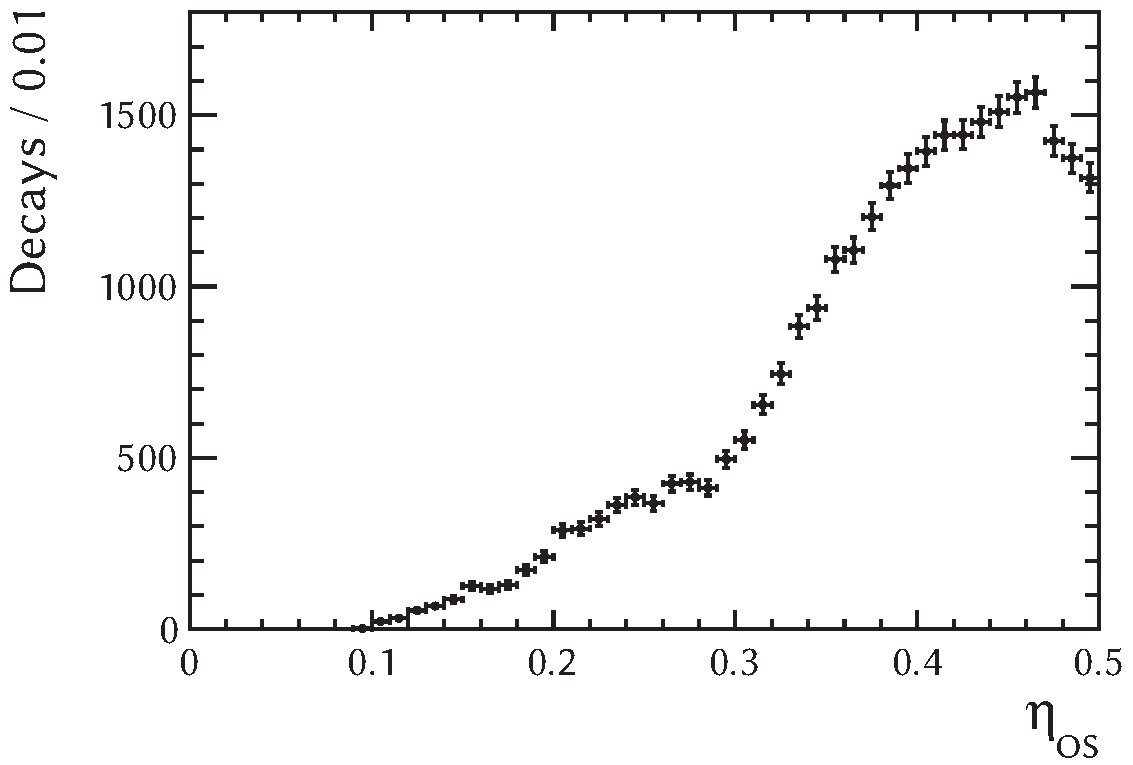
\includegraphics[width=\textwidth]{graphics/analysis/etaOS}
    \caption{}
    \label{fig:etaOS}
  \end{subfigure}%
  \hfill%
  \begin{subfigure}{0.49\textwidth}
    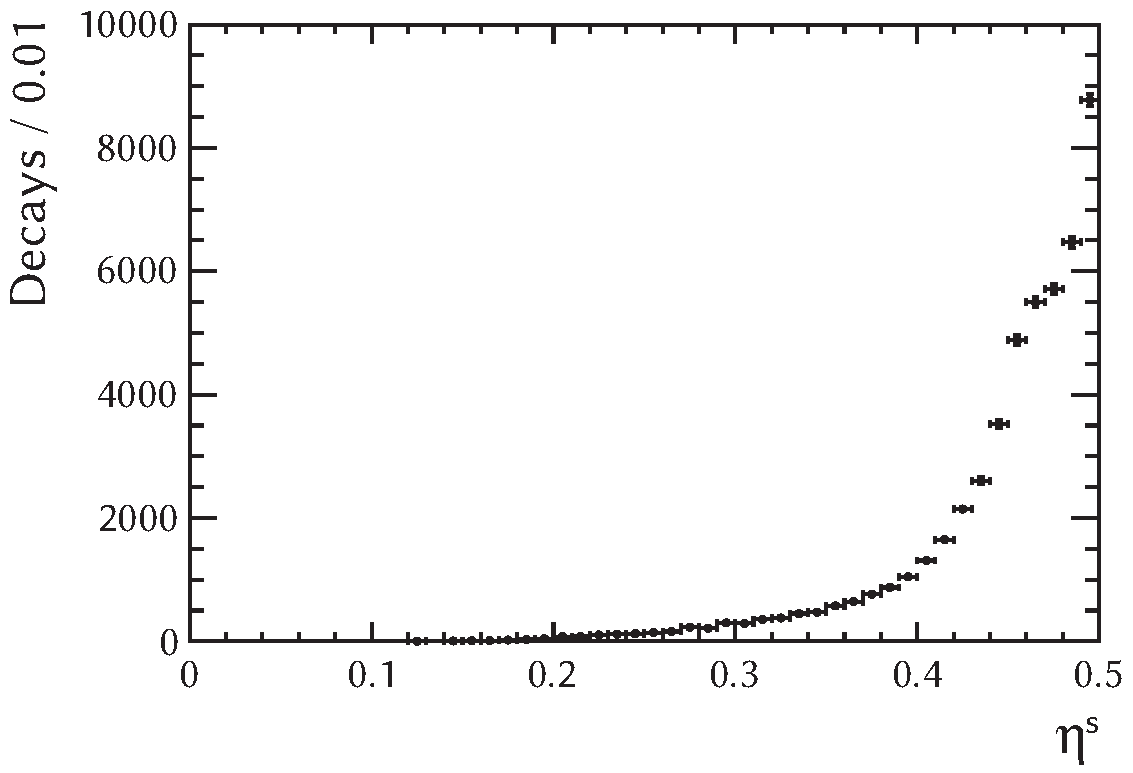
\includegraphics[width=\textwidth]{graphics/analysis/etaSS}
    \caption{}
    \label{fig:etaSS}
  \end{subfigure}
  \caption{Distribution of \BstoJpsiKK{} signal decays in the estimated wrong-tag probability
           for (a) opposite-side tagging and (b) same-side tagging.
           The contributions of untagged decays ($\etaTag$\textequiv0.5) are not shown.}
  \label{fig:etaDists}
\end{figure}

From Figure~\ref{fig:etaDists} it can be seen that although the efficiency of same-side tagging is higher than the efficiency for
opposite-side tagging, the mean wrong-tag probability of the former is closer to 0.5 (``untagged''). As a result, the effective same-side
efficiency is lower than the effective opposite-side efficiency (Table~\ref{tab:tagCats}): 1.2\% for OS-only decays and 0.8\% for SS-only
decays.

Because the oscillatory functions in the ``0$\perp$'' and ``$\parallel\perp$'' interference terms are not proportional to unknown
CP-violation parameters, there is some sensitivity for the value of the tagging dilution in the \BstoJpsiKK{} data. This information is
combined with the value measured in the tagging-calibration procedure by varying the calibration parameters in the fit, constraining them
to the calibration values within uncertainties. The constraints are implemented by adding parabolic terms to the NLL, as for the parameters
$\beta$ of the reconstruction-acceptance function (Section~\ref{subsec:ana_time_acc}).

In practice the calibration parameters $\pTag[i]$ and $\pTagBar[i]$ are not measured directly, but rather their averages and differences,
defined as $\tfrac{1}{2}(\pTag[i]+\pTagBar[i])$ and $\pTag[i]-\pTagBar[i]$, respectively. The values measured after
calibration~\cite{LHCb-ANA-2014-039} and the values from the fit are shown in Table~\ref{tab:tagCalib}. The fit values are only marginally
different from the calibration values, which indicates that the estimates of these parameters in the flavour-tagging procedure are more
precise than the estimates from the \BstoJpsiKK{} data.
\begin{table}[htb]
  \centering
  \caption{Values of tagging-calibration parameters.}
  \label{tab:tagCalib}
  \renewcommand{\arraystretch}{1.1}
  \begin{tabular}{ccc}
    \hline
    parameter                                                 &  calibration value               &  fit value  \\
    \hline
    $\tfrac{1}{2}(\pTag[0][\text{o}]+\pTagBar[0][\text{o}])$  &  \phantom{\tp}0.379\textpm0.004  &  \phantom{\tp}0.381\textpm0.004  \\
    $\tfrac{1}{2}(\pTag[0][\text{s}]+\pTagBar[0][\text{s}])$  &  \phantom{\tp}0.445\textpm0.005  &  \phantom{\tp}0.446\textpm0.005  \\
    $\tfrac{1}{2}(\pTag[1][\text{o}]+\pTagBar[1][\text{o}])$  &  \phantom{\tp}1.00\textpm0.04    &  \phantom{\tp}1.01\textpm0.03    \\
    $\tfrac{1}{2}(\pTag[1][\text{s}]+\pTagBar[1][\text{s}])$  &  \phantom{\tp}1.00\textpm0.09    &  \phantom{\tp}0.97\textpm0.08    \\
    $\pTag[0][\text{o}]-\pTagBar[0][\text{o}]$                &  \tp0.0140\textpm0.0012          &  \tp0.0140\textpm0.0012          \\
    $\pTag[0][\text{s}]-\pTagBar[0][\text{s}]$                &  \tm0.0158\textpm0.0014          &  \tm0.0158\textpm0.0014          \\
    $\pTag[1][\text{o}]-\pTagBar[1][\text{o}]$                &  \tp0.066\textpm0.012            &  \tp0.066\textpm0.012            \\
    $\pTag[1][\text{s}]-\pTagBar[1][\text{s}]$                &  \tp0.008\textpm0.022            &  \tp0.008\textpm0.022            \\
    \hline
  \end{tabular}
\end{table}

An individually normalized PDF is used for each tagging category to be insensitive to the fractions of decays in the categories, for which
there are no predictions. Since also the distributions in estimated wrong-tag probability are unpredicted, the PDFs are also made
conditional on this variable and normalized individually with respect to decay time and decay angles for each combination of $\etaOS$ and
$\etaSS$ values.

The PDFs are also normalized individually for each value of the estimates of the $\Bs$ flavour, $\qtOS$ and $\qtSS$. Although expressions
for the differential decay rates do predict the relative amounts of $\Bs$ tags and $\Bsbar$ tags, a PDF with a common normalization would
be very sensitive to the values of the normalization asymmetries that are used in the model. With individual normalizations this
sensitivity is reduced, which justifies the assumption of no normalization asymmetries (see also Section~\ref{sec:result_syst}).

To demonstrate the sensitivity to normalization asymmetries, the decay-rate equations with one flavour tag
(Equation~\ref{eq:evenOddTagCoefsOneTag}) are considered in the limit of small normalization asymmetries ($\avgCEven$\textapprox1,
$A$\textequiv$\avgCOdd$\textapprox0), large wrong-tag probability ($\dil$\textapprox0), and no wrong-tag asymmetries
($\ADilWTag$\textequiv0):
\begin{equation}
  \left(\frac{\ud^4\Gamma}{\ud t\, \ud\Omega}\right)_{\!\qt}
      \approx (1 + \qt\,A\,\dil)\,\even + (A + \qt\,\dil)\,\odd \ .
\end{equation}

Using individually normalized PDFs for $\qt$\texteq\tp1 and $\qt$\texteq\tm1, an incorrect value of the normalization asymmetry $A$
gives an incorrect estimate of the ``effective dilution factor'' $A$\textpm$\dil$. The effects of this incorrect dilution value on the
estimates of the parameters contained in $\even$ and $\odd$ are expected to roughly cancel between $\qt$\texteq\tp1 and $\qt$\texteq\tm1.

If instead a common normalization is used for $\Bs$ and $\Bsbar$ tags, the distribution of decays in $\qt$ is fitted, which is
approximately given by
\begin{equation}
  P_{\qt}
    \equiv \frac{\int\ud t\, \ud\Omega\left(\frac{\ud^4\Gamma}{\ud t\, \ud\Omega}\right)_{\!\qt}}
                {\sum_{\qt}\int\ud t\, \ud\Omega\left(\frac{\ud^4\Gamma}{\ud t\, \ud\Omega}\right)_{\!\qt}}
    \approx \frac{1}{2}\, \frac{1 + \qt\,A\,\dil + (A + \qt\,\dil)\,R_{\odd/\even}}{1 + A\,R_{\odd/\even}}\ ,
\end{equation}
where $R_{\odd/\even}$ is the ratio of the integrals with respect to time and angles of the $\even$ and $\odd$ terms. As a result, the
analysis is sensitive to the asymmetry between the $\Bs$ and $\Bsbar$ values, approximated by
\begin{equation}
  \frac{P_+ - P_-}{P_+ + P_-} \approx \dil\, \frac{A + R_{\odd/\even}}{1 + A\,R_{\odd/\even}}\ .
\end{equation}
An incorrect estimate of the normalization asymmetry $A$ now directly affects the estimated values of the parameters contained in the ratio
$R_{\odd/\even}$. Since the time integral over the many $\cDms$ and $\sDms$ periods in $\odd$ almost vanishes, which makes $R_{\odd/\even}$
very small by construction, this effect is large and will be avoided by using individually normalized PDFs.
